\documentclass[12pt]{article}

\usepackage[
    %raggedright
]{pimpvanilla}
\usepackage{lipsum}

\title{The \texttt{pimpvanilla} package}
\author{Sylvain Kern}

\begin{document}

\maketitle

\begin{abstract}
    This package is intended to slightly improve the look of vanilla \LaTeX{} --upon my standards-- while remaining as light and versatile as possible.
\end{abstract}

\section{What it looks like}

Like this. \lipsum[1-2]

\section{The font}

The font is \texttt{mlmodern}, a little bit thicker version of Latin Modern. It reduces contrast and makes the text less harsh to read.

\section{Captions}

Captions change a bit, to make them more distinguishable. See figure \ref{fig:juch}.

\begin{figure}
    \centering
    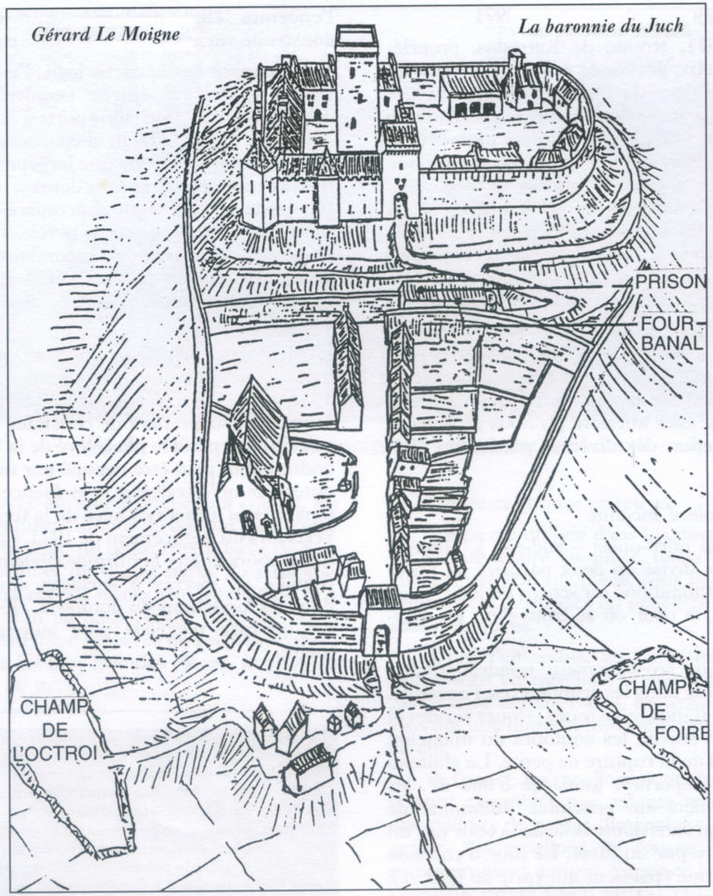
\includegraphics[width=.75\textwidth]{lejuch.png}
    \caption{The famous historical castle of Le Juch, in French Brittany. The family still lives inside. \lipsum[3]\label{fig:juch}}
\end{figure}


\section{Other changes}

Right-justification is slightly improved with the \texttt{microtype} package. Page numbers are now on the left

\end{document}